\section{Introduction}
\label{sec:intro}

Complex systems with a large number of simply interacting pieces underlie many natural processes and, more recently,
have been studied in computer science in an effort to make sense of how simple machine learning algorithms can learn complex structures latent in large, semi-random input data.
Iterative optimization algorithms making sequential updates can be viewed as dynamical systems,
with the main task being to understand how the algorithm evolves over time and what properties the eventual output will have.

When the size of these systems grows very large, a key insight from statistical physics is that 
the macroscopic properties of the system can simplify dramatically:

\begin{quote}
    \textit{As the size of a random, smoothly-interacting dynamical system grows, the effect of individual particles averages out, and the dynamical system's trajectory approximately follows an asymptotic distributional equation.}
\end{quote}

We refer to these distributional equations as \emph{(asymptotic) effective
dynamics}.
We seek to prove this kind of theorem for discrete-time nonlinear iterative algorithms such as those used in modern optimization, statistics, and machine learning.
Concretely, we study \emph{general first-order methods} (GFOM) \cite{celentano2020estimation, montanari2022statistically} which take as input a symmetric matrix $\bA \in \R^{n \times n}$, maintain a vector state $\bmx \in \R^n$, and at each step can perform one of two possible operations:
\begin{enumerate}[1.]
    \item either multiply the state by $\bA$:
        \[ \bmx_{t+1} = \bA \bmx_t\,, \]
    \item or apply a function $f_t : \R^{t+1} \to \R$ componentwise to the previous states:
        \[ \bmx_{t+1} = f_t(\bmx_t, \dots, \bmx_0), \,\,\,\, \text{i.e.,} \,\,\,\, \bmx_{t + 1}[i] = f_t(\bmx_{t}[i], \dots, \bmx_{0}[i]) \text{ for each } i \in [n]\,. \]
\end{enumerate}
The initial state will be either the deterministic all-ones vector $\bmx_0 = \mathbf{1}$, or a random Gaussian vector $\bmx_0 \sim \calN(\mathbf{0}, \bI)$ independent of $\bA$.
Without loss of generality, we may assume that these operations alternate, giving an iteration of the form
\[ \bx_{t + 1} = \bA f_t(\bx_t, \dots, \bx_0)\,. \]
We fix some number of iterations $t$ and view $\bx_t = \bx_t(\bA)$ as the output of the algorithm.

GFOM is a flexible computational model which is expressive enough to capture many types of gradient descent~\cite{celentano2020estimation, gerbelot2022rigorous} and message passing algorithms~\cite{feng2022unifying}.
It may be viewed as a nonlinear version of the power method for estimating top eigenvectors. The alternation of linear and nonlinear steps also closely matches the structure of a feedforward neural network~\cite{cirone2024graph}.
One may view the structural restriction on GFOM as forcing $\bm x_t$ viewed as a function of $\bm A$ to be \emph{permutation-equivariant}: if we apply the same permutation to the rows and columns of $\bm A$, then $\bm x_t$ undergoes the same permutation, a natural condition of an algorithm's not depending on the particular indexing of its inputs.

GFOM and their special case of \emph{approximate message passing} (AMP) are very popular algorithms for many statistical inference tasks and are known to perform optimally in various such settings~\cite{donoho2009message,rangan2011generalized,montanari2012graphical,rangan2016inference,bayati2011dynamics,feng2022unifying}.
In these cases, an algorithm takes as input not an arbitrary matrix $\bA$, but one that contains a corrupted observation of a signal (in a common example, the input $\bA$ is a low-rank $\by\by^{\top}$ plus independent random noise).

GFOM have also been used as optimization algorithms in average-case settings without any such planted structures.
For instance, they are the best known algorithms for optimizing quadratic forms with random coefficients over the non-negative orthant \cite{MR-2015-NonNegative} (the \emph{non-negative PCA} objective function), other convex cones \cite{DMR-2014-ConePCA}, and the hypercube \cite{montanari2021optimization} (the \emph{Sherrington--Kirkpatrick Hamiltonian}), all of which are NP-hard problems in the worst case.
This situation is the main target of our analysis. We receive an input matrix $\bA$ without any particular ``signal'' and wish to output $\bx$ approximately solving an optimization problem parametrized by $\bA$, such as 
\begin{equation}
\label{eq:quad-opt}
\begin{array}{ll} \text{maximize} & \langle \bx, \bA\bx\rangle \\ \text{subject to} & \bx \in S \end{array}
\end{equation}
studied in the above references for various choices of the constraint set $S \subseteq \R^n$.


To view GFOM as an instance of the physical setting sketched above, we consider a growing sequence of matrices $\bA = \bA^{(n)} \in \R^{n \times n}$, and think of the ``particles'' as being the coordinates $\bmx_{t}[i]$ of $\bm x_t \in \R^n$.
To keep notation reasonable, while all of these objects depend on $n$, we omit the $(n)$ superscript whenever possible.
We analyze the \emph{empirical distribution} of our particles, accessed by sampling a random coordinate of a vector:
\[ \samp(\bm x) \colonequals \bmx[i] \in \R \text{ for } i \sim \Unif([n])\,. \]
In order to study a particle's entire trajectory more generally, we may ``stack'' several vectors
and define $\samp((\bx_0, \dots, \bx_t)) := \samp(\bx_0, \dots, \bx_t) \colonequals (\bmx_0[i],\dots, \bmx_t[i]) \in \R^{t + 1}$ for $i \sim \Unif([n])$.

The analysis of GFOM hinges on the observation that these random variables often converge in distribution to certain limiting distributions.
That is, for suitably nice test functions $\varphi: \R^{t + 1} \to \R$,
\[ \lim_{n \to \infty} \E \varphi\big(\samp(\bx_0^{(n)}, \dots, \bm x_t^{(n)})\big) = \lim_{n \to \infty} \E \frac{1}{n} \sum_{i = 1}^n \varphi(\bmx_{0}^{(n)}[i], \dots, \bmx_{t}^{(n)}[i]) = \int \varphi \,\d\nu_{\leq t}^{\infty}\,, \]
for some probability measures $\nu_{\leq t}^{\infty}$.
For example, we can analyze the objective function of a problem like~\cref{eq:quad-opt} in this way: given a GFOM to run for $t$ iterations producing $\bx_t = \bx_t(\bA)$, we extend it to $\bx_{t + 1} = \bA \bx_t$ so that
\[ \E \frac{1}{n}\langle \bx_t, \bA \bx_t\rangle = \EE \frac{1}{n}\langle \bx_t, \bx_{t + 1}\rangle = \EE \frac{1}{n}\sum_{i = 1}^n \bmx_{t}[i] \bmx_{t + 1}[i]\,, \]
a quantity accessible in the above formalism by a suitable choice of $\varphi$.
We can also study the algorithm's convergence by expanding $\frac{1}{n}\|\bx_t - \bx_{t - 1}\|^2_2$ in the same way.

The goal of an asymptotic effective dynamics is then to identify the asymptotic measures $\nu_{\leq t}^{\infty}$\,.
Such a description is a natural first step to designing {\em optimal} GFOM for optimization problems: given an explicit description of the limiting performance of any GFOM, we then optimize the performance over all GFOM~\cite{celentano2020estimation, AMS20:pSpinGlasses, montanari2022equivalence,pesentiThesis}.

The goal of this paper is to study the following three questions regarding effective dynamics:
\begin{enumerate}[1.]
    \item \textbf{Existence:} What are minimal assumptions on the input matrices and the algorithm that ensure the existence of asymptotic effective dynamics?
    \item \textbf{Universality:} What properties of the sequence of input matrices $\bA^{(n)}$ determine the asymptotic effective dynamics?
    In particular, how can we show that two sequences of $\bA^{(n)}$ share the same dynamics?
    \item \textbf{Explicit Calculation:} What are the effective dynamics? In particular, for a given algorithm, how can one describe $\nu_{\leq t}^{\infty}$ for each fixed $t \in \mathbb{N}$?
\end{enumerate}

\subsection{Approximate message passing and simple effective dynamics}

The majority of results to date on effective dynamics for GFOM, including ours, are most useful for \emph{Approximate Message Passing}~(AMP) algorithms. Originating from physicists' work on mean-field spin glass models \cite{mezard1987spinglasstheoryandbeyond,donoho2009message},
AMP algorithms are a special case of GFOM with very simple effective dynamics: each distribution $\nu_t^{\infty}$ (the marginal distribution of $\nu_{\leq t}^{\infty}$ above on the last coordinate) is a Gaussian distribution,
\[ \nu_t^{\infty} = \mathcal{N}(\mu_t, \sigma_t^2)\,, \]
and the effective dynamics gives $(\mu_{t+1}, \sigma_{t+1}^2)$ in terms of $(\mu_{t}, \sigma_{t}^2), \dots, (\mu_{0}, \sigma_0^2)$ via a formula known as the \emph{state evolution} equation.
This gives a simple yet complete description of the leading-order behavior of an algorithm as $n \to \infty$.
In part due to the power afforded by such a description, AMP (and the closely related \emph{belief propagation}, of which AMP is a limit in a suitable sense)
has taken on an indispensable role in statistical physics \cite{mezard1987spinglasstheoryandbeyond, MezardMontanari, charbonneau2023spin} and, more recently, in computational statistics \cite{zdeborova2016statistical, feng2022unifying}.

In fact, while the original appearances of AMP in statistical physics were intrinsically motivated, for statistics applications the simplicity of state evolution is so useful that a line of work has emerged trying to \emph{design} GFOM that have Gaussian $\nu_t^{\infty}$ and effective dynamics given by state evolution~\cite{javanmard2013state,barbierSpatial,vila2015adaptive,fan2022approximate,zhong2024approximate, lovig2025universality}.
The term ``AMP'' is now often used to describe any choice of GFOM for a given family of inputs $\bA^{(n)}$ that has these properties.
While it is not clear that this should be the case \emph{a priori}, a common fortuitous coincidence is that, for various problems, the best GFOM algorithms (in the sense of achieving optimal rates in estimation or inference tasks) happen to be in the special class of AMP.
That is, in many cases, the GFOM with the simplest asymptotic effective dynamics are also the most useful in applications.


Given the successes of AMP, it is a longstanding goal in the literature to identify AMP-like algorithms for as many different choices of inputs and input distributions as possible.
Yet, even to go slightly beyond the simplest choices of matrices $\bA^{(n)}$ has proved challenging and subtle (e.g., random matrices with i.i.d.\ entries~\cite{javanmard2013state, bayati2015universality},
orthogonally invariant distributions~\cite{fan2022approximate}, or
semi-random ensembles~\cite{dudeja2023universality,wang2022universality}).
Constructing AMP algorithms in such settings involves carefully inserting so-called \emph{Onsager correction terms} into the nonlinearities $f_t$ in ways that remain somewhat mysterious yet are crucial to obtain Gaussian limiting behavior.

Here, we will present an approach to the analysis of GFOM that re-derives different existing variants of AMP in a unified way, derives AMP algorithms for new inputs (both random and deterministic), and offers new conceptual insights into the design of these algorithms and into the proof of their asymptotic effective dynamics, in particular giving a clear combinatorial explanation for the Onsager corrections mentioned above.

\subsection{Our contributions: Combinatorial method for GFOM}
\label{sec:results}

We study GFOM
by expressing them as vectors of polynomials in the entries of the input matrix.
For this reason we focus on polynomial $f_t$; it is likely possible to treat more general nonlinearities by approximating them by polynomials (see~\Cref{sec:related} for some discussion).
\begin{definition}
    \label{def:pgfom}
    We call a GFOM as described above a \emph{polynomial GFOM} (pGFOM) if all nonlinearities $f_t: \R^{t + 1} \to \R$ are polynomials.
\end{definition}

Our approach is divided into two parts.
The first is a ``static'' analysis of certain symmetric polynomials in the entries of the input $\bA$.
The second translates this to ``dynamic'' information about vector-valued functions, allowing us to calculate effective dynamics for $O(1)$ iterations of GFOM in a general way.

\subsubsection{Statics of graph polynomials: Traffic distributions and universality}

The basic objects of study for our static analysis are the following \emph{graph polynomials}.
\begin{definition}[Diagram classes]
    We write $\calA = \calA_0$ for the set of finite, undirected, connected (multi)graphs.
    We also write $\calE = \calE_0 \subseteq \calA_0$ for the set of 2-edge-connected (multi)graphs (ones that cannot be disconnected by removing any single edge) and $\calC = \calC_0 \subseteq \calE_0 \subseteq \calA_0$ for the set of \emph{cactus} graphs, ones where every edge belongs to exactly one simple cycle.\footnote{This notion is sometimes more specifically called a \emph{bridgeless cactus}; in this paper we take this to be part of the definition of a cactus.} See~\Cref{fig:cactus}.
\end{definition}
\noindent
The optional subscript ``0'' of the diagram classes refers to the outputs of the polynomials being 0-dimensional, i.e., scalars, which will be useful to distinguish them from vector- and matrix-valued polynomials to be defined later (with subscript ``1'' and ``2'', respectively).

\begin{figure}[ht]
    \centering
    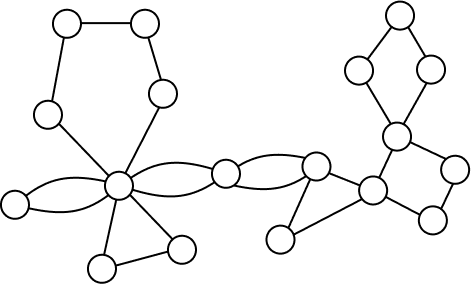
\includegraphics[width=0.4\linewidth]{images/cactus.png}
    \caption{A cactus graph in $\cC$. Intuitively, a cactus is a ``tree of cycles''.}
    \label{fig:cactus}
\end{figure}

\begin{definition}[Scalar graph polynomials]\label{def:w}
    Given $\al \in \calA$ and $\bA \in \R^{n \times n}_{\sym}$\,, define polynomials $w_\al(\bA), z_\al(\bA) \in \R[\bA]$ by:
    \begin{align*}
        w_\al(\bA) &= \sum_{i: V(\al) \to [n]} \prod_{\{u,v\} \in E(\al)} \bA[i(u),i(v)]\,,\\
        z_\al(\bA) &= \sum_{i: V(\al) \embeds [n]} \prod_{\{u,v\} \in E(\al)} \bA[i(u),i(v)]\,.
    \end{align*}
\end{definition}


\noindent That is, $w_\al(\bA)$ and $z_\al(\bA)$ are each multivariate polynomials in the $\frac{n(n + 1)}{2}$ entries on and above the diagonal of the matrix $\bA$
obtained by summing over all labelings of the vertices of $\al$ by $[n] = \{1,2,\dots, n\}$ and with each edge corresponding to an entry of $\bA$.
The only difference between $w_\al(\bA)$ and $z_\al(\bA)$ is that the vertex labeling for $z_\al(\bA)$ is restricted to be injective by the notation $i : V(\al) \embeds [n]$ whereas labels in $w_\al(\bA)$ are allowed to repeat.


Each monomial in the entries of $\bA$ can be represented as a multigraph on $\{1,2,\dots, n\}$.
By summing all monomials with the same ``shape'', the $w_\al(\bA)$ and $z_\al(\bA)$ give two different spanning sets for a subspace of the $S_n$-invariant polynomials in the entries of $\bA$, where $S_n$ acts on $\bA$ by permuting the rows and columns simultaneously.
There are only a few possible distinct shapes for monomials with low degree, so analysis on the $w$ or $z$ polynomials is a highly compressed way to analyze $S_n$-invariant low-degree polynomial functions of $\bA$.

The limiting values of the graph polynomials are a basic set of parameters for the sequence of matrices $\bA^{(n)}$, introduced in random matrix theory by Male \cite{male2020traffic}, who termed them the \emph{traffic distribution}.

\begin{definition}[Traffic distribution]
\label{def:traffic-distribution}
    For a sequence of random\footnote{Deterministic matrices are also allowed just by taking a constant distribution.} matrices $\bA = \bA^{(n)} \in \R^{n \times n}_{\sym}$ we say that
    $\calD: \calA \to \R$ is the \emph{(limiting) traffic distribution} of $\bA$ if 
    \begin{equation}
    \lim_{n \to \infty} \frac{1}{n} \E_\bA w_{\alpha}(\bA) = \calD(\alpha) \text{ for all } \alpha \in \calA. \label{eq:traffic-conv}
    \end{equation}
    We say the (limiting) traffic distribution exists if the limit exists for all $\al \in \calA$.\footnote{
    Note that the diagram $\al$ cannot depend on $n$. It has constant size as $n \to \infty$.
    }
\end{definition}

When the limiting traffic distribution exists, it is easy to show that it determines the
asymptotic behavior of all constant-time GFOM algorithms with input $\bA$:
\begin{claim}
\label{prop:gfom-polynomial}
    Assume that $\bA = \bA^{(n)} \in \R^{n \times n}_{\sym}$ have traffic distribution $\cD$, and that a pGFOM defines $\bx_t = \bx_t(\bA)$ with $\bx_0 = \bm 1$.
    Then, for any fixed $t$ and polynomial $\varphi \in \R[x]$,
    \[ \lim_{n \to \infty} \E_\bA  \frac{1}{n}\sum_{i=1}^n \varphi(\bmx_{t}[i]) = C, \]
    where $C$ is a constant depending only on $\cD$, $(f_s)_{1 \leq s \leq t}$, and $\varphi$.
\end{claim}

Because of this observation, the traffic distribution is a natural way both to show existence of effective dynamics for constant-time GFOM (when the traffic distribution exists then so do effective dynamics) and to characterize the \emph{universality class} of GFOM
(when two sequences of matrices have the same traffic distribution then they have the same effective dynamics).

We now reach our first main contribution: by calculating their limiting traffic distributions, we obtain the first analysis of GFOM on non-trivial completely deterministic inputs.
Namely, we prove that any delocalized orthogonal matrix, after a slight modification, has the same traffic distribution as a corresponding random matrix model, the \emph{regular random orthogonal model} (\rrom; see~\Cref{def:rom}).

\begin{theorem}[See~\Cref{thm:universality-orthogonal}]
    \label{thm:intro-hadamard}
    Let $\bm \Pi = \bm \Pi^{(n)} = \bI - \frac 1n \bm 1 \bm 1^\top$ and $\bH = \bH^{(n)}\in\R_{\sym}^{n\times n}$ be a sequence of orthogonal matrices such that
    \begin{align}
        \max_{1\le i, j\le n} |\bmH[i,j]|\le n^{-\frac 12 + o(1)}\,.\label{eq:delocalization}
    \end{align}
    Then, the traffic distribution of $\mathbf \Pi \bmH \mathbf \Pi$
    exists and equals that of the \rrom.
\end{theorem}
\noindent
The motivating examples for~\cref{thm:intro-hadamard} are ``Fourier transform matrices'' such as the Walsh--Hadamard matrix (\Cref{def:hadamard}), discrete sine transform matrix, or discrete cosine transform matrix (\Cref{def:dst}).
We call conjugating by the projection matrix $\matPi$ \emph{puncturing} the matrix.
\Cref{thm:intro-hadamard} implies
that, after puncturing, the effective dynamics of GFOM
on these matrices are the same as those for the \rrom, which itself is a punctured version of the \emph{random orthogonal model} (\rom) of~\cite{marinari1994replicaI}.
Explicit state evolution equations for these dynamics are given in~\Cref{prop:hadamard-explicit-state}.

Puncturing is necessary in~\Cref{thm:intro-hadamard} and is natural for Fourier transform matrices. For the Walsh--Hadamard matrix, puncturing removes the first row and column, all of whose entries are identically $1/\sqrt{n}$.
This row/column makes $\bH\bm{1}$ have a single large entry; because of that imbalance, without puncturing the traffic distribution of $\bH$ does not exist\footnote{For example, when $\bH$ is the Walsh--Hadamard matrix, the degree-$D$ star diagram $\sigma_D$ satisfies $\frac 1n |w_{\sigma_D}(\bH)| = \Theta(n^{D/2-1})$, which diverges for $D>2$.} and some GFOMs do not have well-defined asymptotic dynamics.
This phenomenon has also been observed experimentally: \cite{schniter2020simple} writes that ``structured matrices (e.g., DCT, Hadamard, Fourier) should work as
well as i.i.d.\ random ones. But, in practice, AMP often diverges with such structured matrices.''
We propose, and our results corroborate, that it is precisely alignment with the all-ones vector that causes this behavior.


Showing that Fourier transform matrices are pseudorandom orthogonal matrices has been a longstanding folklore open problem
in the statistical physics and AMP literature.
It seems to originate in the work of \cite{marinari1994replicaI,marinari1994replicaII,parisi1995mean} in statistical physics, who proposed these matrices as couplings for spin glass models.
Recently (nearly 30 years later),~\cite{dudeja2023universality}
summarized the situation as follows:
\begin{displayquote}
    More generally, numerical studies reported in the literature \emph{[...]}
    suggest that AMP algorithms exhibit universality properties as long as the
    eigenvectors are generic. Formalizing this conjecture remains squarely beyond
    existing techniques, and presents a fascinating challenge.
\end{displayquote}
Similar comments have been made in \cite{subsamplingJavanmard,rangan2019convergence,barbierSpatial}, and relevant numerical experiments can be found in \cite{CO-2019-TAPEquationAMPInvariant,abbara2020universality,dudeja2023universality}. 
Fourier transform matrices are also
favored in compressed sensing applications since they admit fast
multiplications via the Fast Fourier Transform~\cite[Example 2.26]{wang2022universality}.

Although \cref{thm:intro-hadamard} concerns orthogonal 
matrices, we also prove generally that after puncturing, any sequence of delocalized matrices has the same traffic distribution as the orthogonally invariant ensemble with the same eigenvalue distribution, assuming stronger delocalization properties than~\cref{eq:delocalization}. See~\Cref{thm:universality-new} for the formal statement.

\subsubsection{Cactus properties: conditions for simple traffic distributions}

The traffic distribution is a complicated object in general, just because its indexing set $\mathcal{A}$ is very large.
Fortunately, traffic distributions of many common matrices are much simpler.
Specifically, they often satisfy a \emph{cactus property}:
almost all of the graph polynomials $z_\al(\bA)$ are asymptotically negligible as $n \to \infty$, with the only exceptions being the cactus graphs $\al \in \cC \subsetneq \mathcal{A}$ (in the $z$ basis, but \emph{not} in the $w$ basis).

\begin{definition}[Cactus properties and cactus type]\label{def:cactus-property}
    For a sequence of symmetric matrices $\bA = \bA^{(n)} \in \R^{n \times n}$, we say that:
    \begin{enumerate}[(i)]
        \item $\bA$ has the \emph{strong cactus property} if $\lim_{n \to \infty} \frac{1}{n}\E_\bA z_{\alpha}(\bA) = 0$ for all $\alpha \in \calA \setminus \calC$.
        \item $\bA$ has the \emph{weak cactus property} if $\lim_{n \to \infty} \frac{1}{n} \E_\bA z_{\alpha}(\bA) = 0$ for all $\alpha \in \calE \setminus \calC$.
        \item $\bA$ has the \emph{factorizing (strong or weak) cactus property} if it has the (strong or weak) cactus property, and for each $\sig \in \cC$ we have $\lim_{n \to \infty}\frac 1n \E_\bA z_\sig(\bA) = \prod_{\rho \in \cyc(\sig)} \kappa_{|\rho|}$ for some real numbers $\kappa_q$, where $\cyc(\sig)$ is the set of cycles of a cactus and $|\rho|$ is the length of a cycle.\footnote{In the traffic probability literature, the factorizing strong cactus property has been referred to as a traffic distribution being \emph{of cactus type} \cite{cebron2024traffic}. The parameters $\kappa_q$ are the \emph{free cumulants} appearing in free probability theory.}
    \end{enumerate}
\end{definition}

The idea that the non-negligible diagrams for many random matrix models are cactuses appeared in the physics literature as early as the 1990s \cite{parisi1995mean, MFCKMZ-2019-PlefkaExpansionOrthogonalIsing}
and we will show in~\Cref{sec:feynman-physics} how it can be derived from the \emph{Feynman diagram expansion} widely used in physics.
More recent mathematical work~\cite{male2020traffic,cebron2024traffic} reviewed in~\cref{sec:trafficRandom} has rigorously established the strong cactus property for Wigner matrices and unitarily invariant matrices whose eigenvalue distributions converge weakly.
In fact,  
the factorizing strong cactus property is essentially {equivalent} to $\bA$ having the same limiting traffic distribution as some orthogonally invariant random matrix model.

The strong cactus property implies that the traffic distribution is specified only by the limiting values associated to $\sig \in \mathcal{C}$, a much smaller set of graphs than $\mathcal{A}$.
Another way to say this is that, under the strong cactus property, the traffic distribution contains no extra information beyond the considerably simpler \emph{diagonal distribution}, introduced by \cite{wang2022universality}.

\begin{definition}[Diagonal distribution]\label{def:diagonal-distribution}
    For a sequence of symmetric matrices $\bA = \bA^{(n)} \in \R^{n \times n}$, we say that
    $\calD: \calC \to \R$ is the \emph{limiting diagonal distribution} of $\bA$ if
    \[ \lim_{n \to \infty} \frac{1}{n}\E_\bA  w_{\sig}(\bA) = \calD(\sig) \text{ for all } \sig \in \calC. \]
    We say the diagonal distribution exists if the limit exists for all $\sig \in \calC$.
\end{definition}

Let us make several important observations about the definitions of the
traffic distribution, the diagonal distribution, and the cactus
properties.

First, note that~\cref{def:cactus-property} is stated in the $z$-polynomial basis, whereas~\cref{def:traffic-distribution,def:diagonal-distribution} are stated in the $w$-polynomial
basis.
Throughout the paper, it will be helpful to move back and forth
between these bases, since some properties are most natural (or even are
only true) in one basis or the other.
This can be done via M{\"o}bius inversion, as described
in~\Cref{sec:mobius}.

Second, neither the diagonal distribution nor the traffic
distribution is an actual probability distribution.
Instead, they should be interpreted as specifying limiting moments of
certain empirical distributions, namely, the empirical distributions
of the entries of vector graph polynomials.\footnote{
The reason for the name of the diagonal distribution $\calD$ is that it can also be interpreted as specifying the moments of the empirical distribution over the diagonal of certain matrices, namely those that can be formed from $\bA$ by matrix multiplication and the operation of zeroing out the off-diagonal entries of a matrix \cite{wang2022universality}.}

Third, one can view the diagonal and traffic distributions as
generalizations of the limiting spectral distribution of a sequence of matrices.
The spectral moments are $\frac1n \Tr(\bA^q)=\frac1n w_\alpha(\bA)$,
where $\alpha$ is the $q$-cycle diagram, so they are included in both
the diagonal and traffic distributions:
\[ \text{`` spectral distribution} \,\, \subsetneq \,\, \text{diagonal distribution} \,\, \subsetneq \,\, \text{traffic distribution ''} \]

Just as the empirical spectral distribution characterizes the
limiting behavior of all polynomials in $\bA$ that are invariant under
the action of the orthogonal group $O(n)$
(acting by $\bQ \cdot \bA = \bQ\bA\bQ^{\top}$), the traffic distribution characterizes the limiting behavior of the larger space of
polynomials invariant under the smaller symmetric group
$S_n$, i.e.,\ where $\bQ$ is restricted to be a permutation matrix.

Finally, the strong cactus properties describe when these inclusions can
be reversed:
if the strong cactus property holds, then the traffic distribution
contains no more information than the diagonal distribution. If the
factorizing strong cactus property holds, then the diagonal
distribution, in turn, contains no more information than the spectral
distribution.

Due to the effect of the puncturing operation, the strong cactus property actually is \emph{not} satisfied by the pseudorandom
matrices or \rrom matrices appearing in our~\Cref{thm:intro-hadamard}.
But, these matrices satisfy the weak cactus property,
and establishing this is a key step in the analysis of these matrices (in fact, the weak cactus property holds for the Fourier transform matrices without puncturing, as we show in Part 1 of \cref{thm:universality-new}).

\subsubsection{Dynamics of graph polynomials: asymptotic GFOM state and treelike AMP}

Recall that our final goal is to describe the state $\bm x_t = \bm x_t(\bm A)$ of a GFOM.
Since $\bm x_t \in \R^n$ we use vector diagrams for this task.
Compared to the scalar diagrams in $\cA_0$, the only extra information in these diagrams is that one of the vertices is specially marked as the ``root'', whose label specifies the coordinate of the vector output.

\begin{definition}[Vector diagram classes]
    We write $\cA_1$ and $\cC_1$ for the set of graphs in $\cA$ and $\cC$ respectively, further decorated with a distinguished root vertex.
    For $\alpha \in \cA_1$, we write $\rt(\alpha) \in V(\alpha)$ for its root vertex.
\end{definition}

\begin{definition}[Vector graph polynomials]
        Given $\al \in \calA_1$ and $\bA \in \R^{n \times n}_{\sym}$\,, define vectors of polynomials $w_\al(\bA), z_\al(\bA) \in (\R[\bm A])^n$ by,
    \begin{align*}
        \bm w_\al(\bA)[i] &\defeq \sum_{\substack{j: V(\al) \to [n] \\ j(\rt(\al)) = i}} \prod_{\{u,v\} \in E(\al)} \bA[j(u),j(v)]\,,\\
        \bm z_\al(\bA)[i] &\defeq \sum_{\substack{j: V(\al) \embeds [n] \\ j(\rt(\al)) = i}} \prod_{\{u,v\} \in E(\al)} \bA[j(u),j(v)]\,,
    \end{align*}
    for all $i\in [n]$.
\end{definition}

To analyze the vector graph polynomials, we compute the moments of the empirical distribution of their entries.
We will see that these are matched (asymptotically) by a family of scalar random variables $Z_{\alpha}^{\infty}$, so the empirical distribution of the entries of $\bm z_{\alpha}(\bA)$ converges in a suitable sense to $Z_\al^\infty$ as $n\to\infty$.
Further, when $\bA$ has the strong cactus property, an analogous property is inherited by these limiting distributions, only a small number of $\alpha \in \cA_1$ having a non-negligible limit.
\begin{definition}[Treelike diagrams]\label{def:treelike}
    We say that $\alpha \in \cA_1$ is \emph{treelike} if it is a tree with \emph{hanging cactuses} attached to the leaves of the tree (see~\Cref{fig:treelike}).
    We denote the set of treelike diagrams by $\cT_1$, and denote by $\cG_1 \subseteq \cT_1$ the set of treelike diagrams in which, after removing
    hanging cactuses, the root has degree exactly 1. 
\end{definition}

\begin{figure}[ht]
    \centering

    \begin{subfigure}[t]{0.31\linewidth}
        \centering
        \begin{minipage}[c][1.8in][c]{\linewidth}
            \centering
            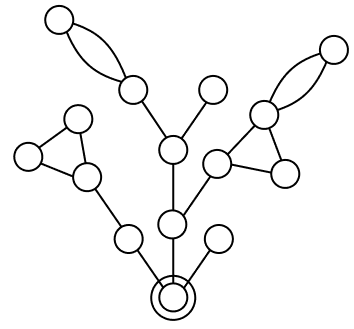
\includegraphics[height=1.8in]{images/hermite-treelike.png}
        \end{minipage}
        \caption{A treelike diagram in $\calT_1$}
    \end{subfigure}
    \hfill
    \begin{subfigure}[t]{0.31\linewidth}
        \centering
        \begin{minipage}[c][1.8in][c]{\linewidth}
            \centering
            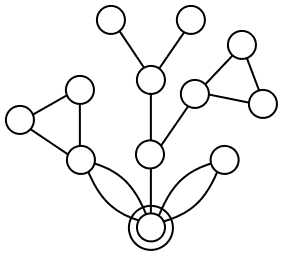
\includegraphics[height=1.5in]{images/treelike.png}
        \end{minipage}
        \caption{A Gaussian diagram in $\calG_1$}
    \end{subfigure}
    \hfill
    \begin{subfigure}[t]{0.31\linewidth}
        \centering
        \begin{minipage}[c][1.8in][c]{\linewidth}
            \centering
            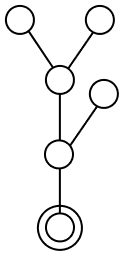
\includegraphics[height=1.5in]{images/tree.png}
        \end{minipage}
        \caption{The diagram in $\calG_1$ after removing its hanging cactus.}
    \end{subfigure}

    \caption{Examples of treelike and Gaussian diagrams. The root vertex is
    circled.}
    \label{fig:treelike}
\end{figure}

\begin{theorem}[Vector polynomial limits; see~\cref{thm:convergence-distribution}]
\label{prop:convergence-distribution}
    Assume that $\bA = \bA^{(n)}$ has the strong cactus property with limiting diagonal distribution $\cD$. 
    Assume also that the sequence of random variables 
    $(\|\bm A^{(n)}\|)_{n\ge 1}$ is \emph{tight},\footnote{If the matrices $\bm A^{(n)}$ are deterministic, this should be understood as $(\|\bm A^{(n)}\|)_{n\ge 1}$ being bounded.} i.e., that
    \begin{equation}
        \text{for all } \varepsilon > 0 \text{ there exists } K > 0 \text{ such that } \sup_{n\ge 1}\Pr(\|\bA^{(n)}\|>K)\le \varepsilon\,.\label{eq:tightnessNorm}
    \end{equation}
    Write $\bz_{\cA_1}(\bA) \in (\R^{\cA_1})^n$ for the stacking of values of all $\bz_{\alpha}(\bA)$ for $\alpha \in \cA_1$.
    Then,
    \[ \samp(\bz_{\cA_1}(\bA)) \xrightarrow[n \to \infty] {\textnormal{(d)}} (Z_{\alpha}^{\infty})_{\alpha \in \cA_1}\,, \]
    for a family of (partially dependent) random variables $(Z_{\alpha}^{\infty})_{\alpha \in \cA_1}$ such that $Z_{\alpha}^{\infty} = 0$ for all $\alpha$ not treelike, and which can be sampled as follows for $\al \in \calT_1$:
    \begin{enumerate}
        \item Draw $(Z_{\sig}^{\infty})_{\sig \in \cC_1}$ from a distribution determined by $\cD$.
        \item Draw $(Z_{\gamma}^{\infty})_{\gamma \in \cG_1} \sim \calN(\bm 0, \bm\Sigma^\infty)$ from a centered Gaussian distribution with countably infinite covariance matrix $\bm\Sigma^\infty$ depending on $(Z_{\sigma}^{\infty})_{\sigma\in\calC_1}$.
        \item Set $(Z_{\alpha}^{\infty})_{\alpha \in \cT_1  \setminus (\cG_1 \cup \cC_1)}$ to be certain deterministic polynomial functions of $(Z_{\alpha}^{\infty})_{\alpha\in \calG_1\cup \calC_1}$.
    \end{enumerate}
\end{theorem}
\noindent
We note that $\samp(\bz_{\cA_1}(\bA))$ is a random variable taking values in $\R^{\cA_1}$, a countable product space.
Thus, its convergence in distribution is the same as convergence in distribution of any finite-dimensional projection; see~\Cref{sec:convergence-process}.

The application to pGFOM is as follows.
Analogously to~\Cref{prop:gfom-polynomial},
it is easy to see that the iterates $\bmx_t(\bmA)$
of a pGFOM admit a diagrammatic expansion
of the form
\begin{equation}
\bm x_t(\bm A) = \sum_{\alpha \in \cA_1} c_{t, \alpha} \bm z_{\alpha}(\bm A)\,, \label{eq:z-expansion-of-x}
\end{equation}
for finitely supported coefficients
$(c_{t,\alpha})_{\alpha\in\calA_1}$.
Given the limits of the individual diagrams above, for a given GFOM, number of iterations $t$, and coefficients as in~\cref{eq:z-expansion-of-x}, we write
\begin{equation*}
    (X_0^{\infty}, \dots, X_t^{\infty}) \defeq \left(\sum_{\alpha \in \cA_1} c_{0, \alpha} Z_{\alpha}^{\infty}, \dots, \sum_{\alpha \in \cA_1} c_{t, \alpha} Z_{\alpha}^{\infty}\right)\,,\label{eq:asymptoticStateIntro}
\end{equation*}
a random variable in $\R^{t + 1}$ that describes the joint empirical distribution of the first $t$ steps of the GFOM.
We call this the \emph{asymptotic state} of a GFOM (\Cref{def:asymptotic-state}). By~\Cref{prop:convergence-distribution}, the asymptotic state describes limiting empirical averages over the GFOM states, in the sense that
\[ \lim_{n \to \infty} \E_{\bA} \frac{1}{n}\sum_{i = 1}^n  \varphi(\bx_0[i], \dots, \bx_t[i]) = \EE\, \varphi(X_{0}^{\infty}, \dots, X_t^{\infty}) \]
for any $\varphi: \R^{t + 1} \to \R$ either a polynomial or a bounded continuous function (\Cref{claim:cvImpliesState}).

In particular, if the only nonzero $c_{t, \alpha}$ in~\cref{eq:z-expansion-of-x} are non-treelike $\al$ or treelike $\alpha \in \cG_1$, then the GFOM has an asymptotic state that is Gaussian conditional on $(Z_{\sigma}^{\infty})_{\sigma\in\calC_1}$.
This observation leads to our second main contribution: a new family of \emph{treelike AMP} algorithms simultaneously generalizing Orthogonal Approximate Message Passing (OAMP) algorithms~\cite{rangan2019vector, fan2022approximate} for orthogonally invariant matrices, and Generalized Approximate Message Passing (GAMP) algorithms~\cite{rangan2011generalized, javanmard2013state} for matrices with independent entries that are not necessarily identically distributed.\footnote{The second comparison is with the caveat that GAMP uses a certain class of ``non-separable'' nonlinearities (applying a different function $f_t$ to each coordinate of $\bmx_t$) which are not directly covered by our result \cite{rangan2011generalized, javanmard2013state}.}

\begin{theorem}[Treelike AMP; see~\Cref{thm:full-onsager}]
\label{thm:intro-onsager}
    Assume that $\bA = \bA^{(n)}$ satisfies the assumptions of \Cref{prop:convergence-distribution}.
    Given polynomial functions $f_t : \R \to \R$, define the pGFOM:
    \begin{equation*}
    %\label{eq:gamp}
    \begin{alignedat}{2}
        &\bmx_0 \defeq \bm{1}\,, \qquad
        &&\bmx_t \defeq \bA \bmf_{t-1}
          - \sum_{s=0}^{t-1}\bmb_{s,t} \cdot \bmf_s \,,
          \qquad
          \text{(The product $\bmb_{s,t} \cdot \bmf_s$ is entrywise.)}
        \\
        &\bmf_t \defeq f_t(\bmx_t)\,, \qquad
        &&\bmf'_t \defeq f'_t(\bmx_t)\,.
    \end{alignedat}
    \end{equation*}
    \begin{equation*}
    \begin{aligned}
        \bmb_{s,t}[i]
        &\defeq
        \sum_{\substack{
            i_s,\dots,i_{t-1}=1\\
            \textnormal{distinct}\\
            i_s=i
        }}^n
        \bA[i_s,i_{t-1}] \bmf'_{t-1}[i_{t-1}]
        \bA[i_{t-1},i_{t-2}] \bmf'_{t-2}[i_{t-2}]
        \cdots
        \bmf'_{s+1}[i_{s+1}]
        \bA[i_{s+1},i_s]\,.
    \end{aligned}
    \end{equation*}
    Then, for any fixed $t$ as $n \to \infty$, the asymptotic state $(X^\infty_1,\ldots,X^\infty_t)$, conditional on $(Z_{\sigma}^{\infty})_{\sigma\in\calC_1}$, is a centered Gaussian vector.
    A formula for its covariance is given in~\cref{lem:cov-cactus}.
\end{theorem}

The subtracted terms $\sum_{s=0}^{t-1} \bm b_{s,t} \cdot \bm f_s$ generalize the ``Onsager correction terms'' appearing in different variants of AMP.
\cref{thm:intro-onsager} and its proof address two questions posed in~\cite{wang2022universality},
namely (1)~to obtain a combinatorial interpretation of the Onsager correction for OAMP algorithms,
and (2)~to identify a more general class of AMP algorithms whose state evolution is characterized by the diagonal distribution of the input matrix.
\cref{thm:intro-onsager} shows that (2) is possible for arbitrary matrices satisfying the strong cactus property, and explicitly describes such an algorithm and its conditionally Gaussian asymptotic states. We
show in~\Cref{sec:se-examples} how the treelike
AMP iteration simultaneously generalizes several
variants of AMP introduced in prior work.

We emphasize that, in contrast to all existing state evolution results we are aware of, we derive an Onsager correction and state evolution formula \emph{without assuming an explicit random model for $\bA$}.
The iteration in~\Cref{thm:intro-onsager} is the same regardless of the limiting diagonal distribution of $\bA$, provided that these matrices (random or deterministic) satisfy the strong cactus property and have \emph{some} limiting diagonal distribution (which will affect the covariance formula in~\cref{lem:cov-cactus}).
Note that the matrices in our universality result (\cref{thm:intro-hadamard}) and their random counterparts (the \rrom), satisfy the weak cactus property instead of the strong cactus one.
Nevertheless, the Onsager correction and the state evolution can still be determined by a reduction to the strong-cactus-property setting, as we explain in~\Cref{sec:dynamics-reg}.

\subsection{Related work}
\label{sec:related}

\paragraph{Moment method for AMP.}
Our overall approach to graph polynomials generalizes prior work for the case of Wigner matrices~\cite{jones2025fourier}.
Similar techniques have also appeared in prior works using the moment method to study AMP algorithms~\cite{bayati2015universality, wang2022universality, montanari2022equivalence, dudeja2023universality, ivkov2023semidefinite, dudeja2024spectral}.
The $w$ and $z$ polynomials are rather fundamental objects which,
along with their vector, matrix, and tensor generalizations,
have variously been called
``graph monomials'' or ``traffics'' in free probability,
``graph matrices'' in computer science,
``graph homomorphism polynomials'' in combinatorics,
and are also related to ``tensor networks'' and ``Feynman diagrams'' in physics.

\paragraph{Polynomial vs.\ non-polynomial GFOM.}
    In random and semi-random models, general
    first-order methods with a constant number of
    iterations using (1) only polynomial
    nonlinearities or (2) arbitrary Lipschitz
    nonlinearities are generally 
    expected to have the same
    computational power. Using polynomial approximation arguments, this has been
    made precise in several previous works~\cite{montanari2022equivalence,ivkov2023semidefinite,wang2022universality}. For example,
    \cite[Lemma 2.12]{wang2022universality} gives
    an abstract reduction
    showing
    that if state evolution for AMP on rotationally-invariant matrices holds for polynomial
    nonlinearities, then it also
    holds for arbitrary Lipschitz nonlinearities.
    While we study more general matrix models, we expect the assumption of polynomial nonlinearities is not essential.


\paragraph{AMP vs.\ GFOM.}
A simple reduction shows that every algorithm in the GFOM class can be expressed as a certain post-processing of an AMP algorithm (allowing ``memory terms'')~\cite{celentano2020estimation}.
Therefore, these two classes of algorithms are equivalent from the standpoint of computational power.
In our analysis, this is mirrored by the fact that, in~\Cref{prop:convergence-distribution}, all possible non-Gaussian limits after conditioning on the draw of $(Z^\infty_{\sigma})_{\sigma\in \calC_1}$ are  deterministic functions of the possible Gaussian limits.

\paragraph{GFOM on independent entry matrices.}
The analysis of GFOM and AMP on Wigner matrices or inhomogeneous versions thereof was the first case widely considered in the literature, and goes back to the origins of the mathematical analysis of AMP in the statistical physics literature on spin glasses~\cite{bolthausen2014iterative,donoho2009message,bayati2011dynamics,montanari2012graphical,barbierSpatial,rush2018finite,LW-2022-NonAsymptoticAMPSpiked}. See~\cite{feng2022unifying} for a survey of many of these works.
Further, see~\cite{bayati2015universality,chen2021universality} for universality results over such models allowing for different entry distributions (but still requiring entrywise independence),~\cite{donoho2013information,javanmard2013state} for results on block-structured variance profiles along the lines of our block GOE model, and~\cite{gueddari2025approximate,bao2025leave} for recent progress on more general variance profiles.

\paragraph{GFOM on orthogonally invariant matrices.} The correct form of AMP (to ensure Gaussian limiting distributions)
in orthogonally invariant models was first predicted non-rigorously for physics applications by~\cite{opper2016theory} using dynamical mean-field theory (DMFT), and then proved by~\cite{fan2022approximate}. Precursors for special ``divergence-free'' forms of AMP were also obtained by~\cite{CO-2019-TAPEquationAMPInvariant,ma2017orthogonal,rangan2019vector,takeuchi2019rigorous} under the names of \emph{Vector AMP} and \emph{Orthogonal AMP}.
Related calculations for a more general statistical physics framework subsuming these AMP variants are carried out in~\cite{MFCKMZ-2019-PlefkaExpansionOrthogonalIsing}; in particular, this work includes special cases of and discusses the more general form of the calculations we detail in~\Cref{app:weingarten}.
See the discussion in~\cite{fan2022approximate} for a more thorough overview of these distinctions.

\paragraph{Universality principles for GFOM.}
Beyond the above results, the main ones we are aware of that reduce the amount of randomness required for AMP are the recent works ~\cite{wang2022universality,dudeja2023universality}, which, modulo technical differences, both prove universality results over random matrices whose distribution is invariant under signed permutations.
In other words, they treat broad classes of matrices provided that these are conjugated by random signed permutations, a considerable reduction in randomness from, e.g., conjugating by random Haar-distributed orthogonal or unitary matrices as in OAMP.
Numerous experimental works have found universality phenomena for ``sufficiently pseudorandom'' deterministic matrices, but we are not aware of any rigorous results for completely deterministic matrices prior to our work.
See discussion in \cite{CO-2019-TAPEquationAMPInvariant,schniter2020simple,abbara2020universality,dudeja2023universality}.

\subsection{Organization of the paper}


We give preliminaries on the matrices considered
in this work and modes of convergence for
our limiting theorem in~\Cref{sec:prelims}.
We introduce our definitions of diagrams and
consequences of M{\"o}bius inversions for the
traffic distribution in~\Cref{sec:diagrams}. In~\Cref{sec:trafficRandom}, to build intuition on
traffic distributions,
we describe them for several random matrix 
ensembles.
\Cref{sec:universality} is dedicated to the proof
of our first main result, the polynomial
universality of delocalized deterministic matrices (\Cref{thm:intro-hadamard}).
\Cref{sec:dynamics} details and proves
the effective dynamics of GFOM under the 
strong cactus property (\Cref{prop:convergence-distribution,thm:intro-onsager}).

We illustrate
two viable approaches to computing the 
traffic distribution
of orthogonally invariant matrix models:~\Cref{sec:feynman-physics} is based on Feynman
diagrams and~\Cref{app:weingarten} relies on
Weingarten calculus. \Cref{sec:convergence-process} provides background on convergence
of stochastic processes, and~\Cref{sec:omitted} contains omitted proofs.


\subsection{Acknowledgments}

Thanks to Zhou Fan, Cynthia Rush, and Subhabrata Sen for helpful discussions over the course of this project.
CJ was supported in part by the European Research Council (ERC) under the European Union's Horizon 2020 research and innovation programme (grant agreement No.
101019547).
LP's work was supported by the Swiss National Science Foundation (SNSF), grant no. 10004947.